\vspace{-0.1in}
\begin{figure}[t]
    \centering
    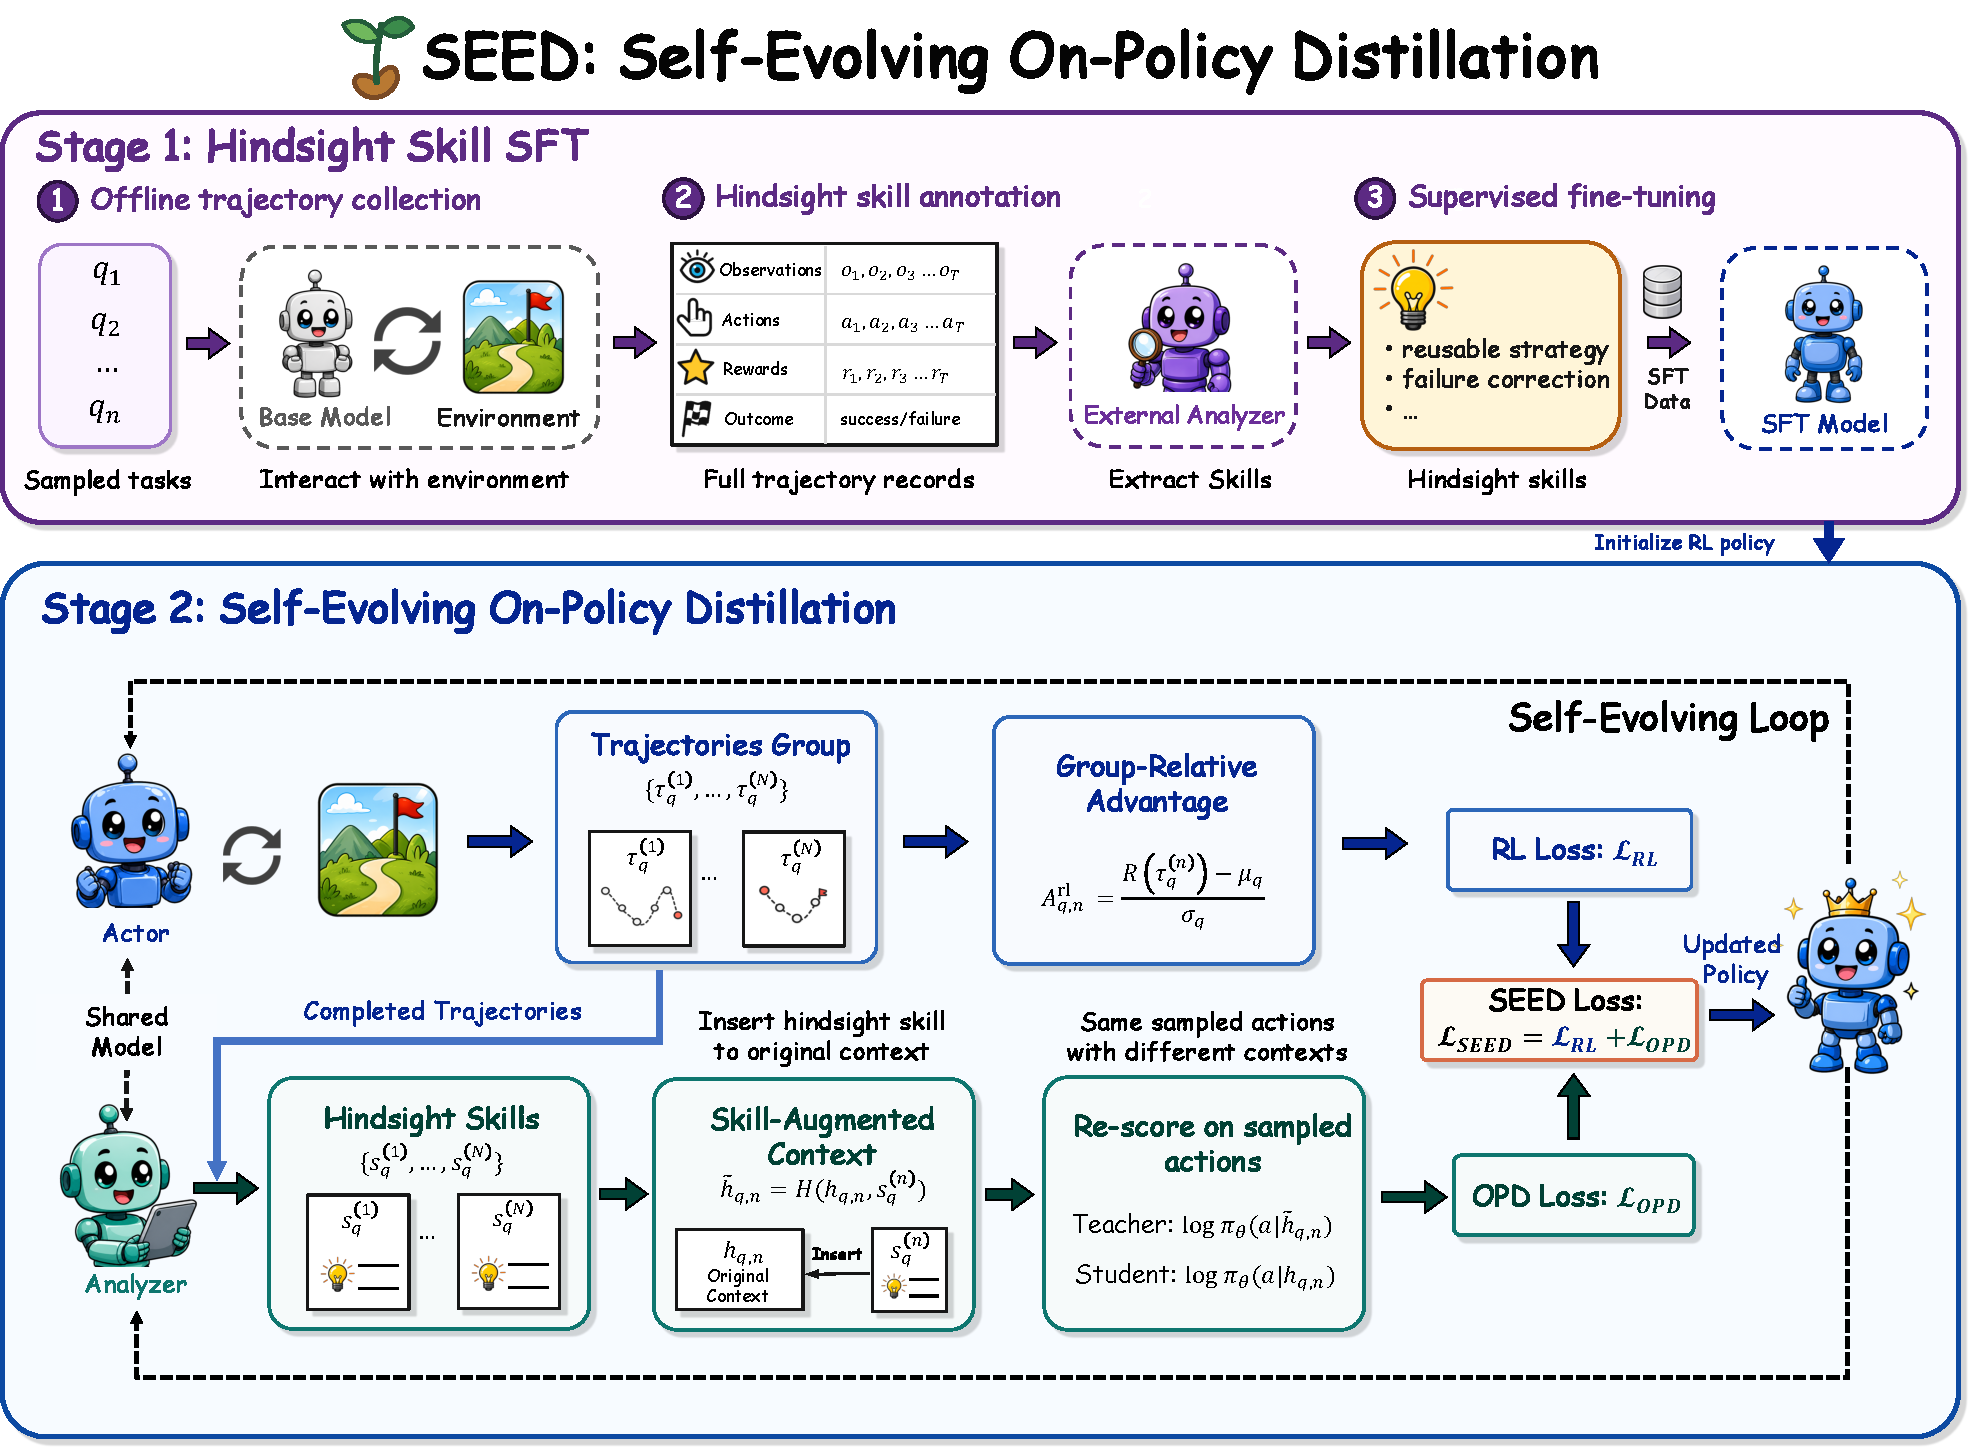
\includegraphics[width=0.96\linewidth]{figures/SEED_framework.pdf}
    \caption{\textbf{Overview of \textsc{Seed}.} \textbf{Stage 1} (Hindsight Skill SFT) equips the policy to extract hindsight skills from completed trajectories. \textbf{Stage 2} (Self-Evolving On-Policy Distillation) jointly optimizes outcome-based RL and skill-conditioned OPD in a self-evolving agentic loop.}
    \label{fig:overview}
    \vspace{-0.1in}
\end{figure}

\section{Method}
We present \textbf{\textsc{Seed}}, a self-evolving OPD framework for agentic RL. \textsc{Seed} is motivated by the observation that completed agent trajectories contain rich hindsight information: even when reward is sparse, a full trajectory often reveals useful behavioral patterns, failure causes, and reusable strategies that are not directly available at intermediate decision steps. \textsc{Seed} converts such hindsight information into \textbf{hindsight skills} and distills their behavioral effect back into the ordinary policy.

As shown in Figure~\ref{fig:overview}, \textsc{Seed} has two training stages. First, hindsight-skill supervised fine-tuning (SFT) equips a single policy model to analyze completed trajectories. Second, the current policy snapshot both collects on-policy trajectories and analyzes them into hindsight skills. The same sampled actions are then re-scored under ordinary and skill-augmented contexts to construct a token-level OPD signal, which is optimized jointly with RL. At inference time, \textsc{Seed} removes the analyzer, so deployment requires only the learned policy.

\subsection{Problem Formulation}
% We formulate long-horizon agentic tasks as partially observable decision processes:
We formulate long-horizon agentic tasks as partially observable Markov decision processes:
\[
\left(
\mathcal{S},
\mathcal{A},
\mathcal{O},
\mathcal{T},
\Omega,
\mathcal{R},
\gamma
\right),
\]
where $\mathcal{S}$ is the latent state space, $\mathcal{A}$ is the action space, $\mathcal{O}$ is the observation space, $\mathcal{T}$ is the transition kernel, $\Omega$ is the observation kernel, $\mathcal{R}$ is the reward function, and $\gamma$ is the discount factor. At timestep $t$, the agent receives an observation $o_t \in \mathcal{O}$ and maintains an interaction history
\[
h_t =
\left(
o_0, a_0, o_1, a_1, \ldots, o_t
\right),
\]
where $a_i$ denotes the textual response or executable action produced by the agent. The policy generates the next action according to
\[
a_t
\sim
\pi_\theta
\left(
\cdot \mid h_t
\right).
\]

A completed trajectory is denoted by
\[
\tau =
\left\{
(o_t, a_t, r_t)
\right\}_{t=0}^{T-1},
\]
with an episode-level outcome $R(\tau) \in \mathbb{R}$. In many agentic environments, $R(\tau)$ is sparse and becomes available only after task completion, such as a binary success indicator or a final task score. The standard reinforcement learning objective is
\[
J(\theta)
=
\mathbb{E}_{\tau \sim \pi_\theta}
\left[
R(\tau)
\right].
\]
This formulation exposes a key challenge in long-horizon agentic RL: the environment provides only trajectory-level feedback, while the policy must learn from many token-level decisions distributed across the interaction history. \textsc{Seed} bridges this granularity gap by deriving an auxiliary training-time token-level signal from hindsight skills extracted after trajectory completion.

\subsection{Hindsight Skill Supervised Fine-Tuning}
The first stage initializes the policy with the ability to analyze full interaction histories and express reusable behavioral guidance as natural-language hindsight skills.

\paragraph{Offline trajectory collection.}
We first collect an offline pool of trajectories using a base policy without skill augmentation. Let $\mathcal{Q}_{\mathrm{sft}} = \{q_j\}_{j=1}^{M}$ be a set of training tasks. For each task $q_j$, we run $K_0$ rollouts with the base policy $\pi_{\theta_{\mathrm{base}}}$:
\[
\mathcal{B}_j
=
\left\{
\tau_{j,k}
\right\}_{k=1}^{K_0},
\qquad
\tau_{j,k}
\sim
\pi_{\theta_{\mathrm{base}}}
\left(
\cdot \mid q_j
\right).
\]
The complete offline trajectory pool is
\[
\mathcal{B}
=
\bigcup_{j=1}^{M}
\mathcal{B}_j.
\]
Each trajectory contains the task description, observations, actions, rewards, and final outcome. These trajectories are collected without any hindsight skill in the decision context, ensuring that the SFT data are derived from ordinary agent-environment interaction.

\paragraph{Hindsight skill annotation.}
Given a completed trajectory $\tau$, an external analyzer $A_{\mathrm{ext}}$ produces a hindsight-skill annotation:
% \[
% s_\tau
% =
% A
% \left(
% \tau
% \right),
% \]
\[
s_\tau
=
A_{\mathrm{ext}}
\left(
\tau
\right),
\]
where $s_\tau$ denotes the skill annotation produced from trajectory $\tau$. For a successful trajectory, $s_{\tau}$ typically captures reusable strategies or workflows that contributed to task completion. For a failed trajectory, $s_\tau$ can encode corrective or avoidance guidance inferred from the observed failure.

We retain the annotation only if the generated skill is correctly formatted. Let $v_\tau \in \{0,1\}$ denote the validity indicator. The accepted SFT set is
\[
\mathcal{D}_{\mathrm{sft}}
=
\left\{
(x_\tau, s_\tau)
:
\tau \in \mathcal{B},
v_\tau = 1
\right\},
\]
where $x_\tau$ is the serialized trajectory-analysis input and $s_\tau$ is the corresponding hindsight skill target.

\paragraph{Supervised fine-tuning.}
We then fine-tune the policy model to predict the hindsight skill from the completed trajectory. The same autoregressive model later initializes both the RL actor and the synchronized trajectory analyzer. For an accepted SFT example $(x_\tau, s_\tau) \in \mathcal{D}_{\mathrm{sft}}$, the model is optimized with the standard negative log-likelihood objective:
\[
\mathcal{L}_{\mathrm{sft}}(\theta)
=
-
\mathbb{E}_{(x_\tau,s_\tau)\sim\mathcal{D}_{\mathrm{sft}}}
\left[
\sum_{\ell=1}^{|s_\tau|}
\log \pi_\theta\!\left(
s_{\tau,\ell}
\mid
x_\tau, s_{\tau,<\ell}
\right)
\right],
\]
where $s_{\tau,\ell}$ is the $\ell$-th token of $s_\tau$. The resulting checkpoint $\theta_{\mathrm{sft}}$ initializes the later RL policy.

During RL, the trajectory analyzer is instantiated directly from the current policy checkpoint. Thus, the same model can act in the environment under ordinary interaction histories and generate hindsight skills from completed trajectories, without a separately trained analyzer.

\subsection{Self-Evolving On-Policy Distillation}
The second stage performs agentic RL with an additional token-level OPD signal. At the start of each update, \textsc{Seed} freezes the current policy as $\pi_{\theta_{\mathrm{old}}}$. This snapshot collects trajectories and also parameterizes the analyzer that extracts their hindsight skills. A trainable policy $\pi_\theta$, initialized from $\pi_{\theta_{\mathrm{old}}}$, is then optimized with both the environment-driven GRPO and OPD objectives. After the update, the optimized policy $\pi_\theta$ becomes the policy snapshot for the next iteration.

This design keeps the distillation signal on-policy: the policy collects its own trajectories, the analyzer agent converts these completed trajectories into hindsight skills, and the behavioral effect of such hindsight guidance is distilled back into the ordinary policy.

\paragraph{On-policy hindsight skill generation.}
For each task prompt $q$, \textsc{Seed} samples a group of $N$ trajectories using the frozen policy:
\[
\mathcal{G}_q
=
\left\{
\tau_q^{(1)}, \tau_q^{(2)}, \ldots, \tau_q^{(N)}
\right\},
\qquad
\tau_q^{(n)}
\sim
\pi_{\theta_{\mathrm{old}}}
\left(
\cdot \mid q
\right).
\]
For each completed trajectory $\tau_q^{(n)}$, \textsc{Seed} constructs its trajectory-analysis input $x_{\tau_q^{(n)}}$. The analyzer agent instantiated from the same policy snapshot $\pi_{\theta_{\mathrm{old}}}$ then analyzes the completed trajectory and generates a hindsight skill:
\[
s_q^{(n)}
=
A_{\theta_{\mathrm{old}}}
\left(
x_{\tau_q^{(n)}}
\right),
\]
where $A_{\theta_{\mathrm{old}}}$ denotes the analyzer role of the shared model. Although the actor and analyzer share the same parameters at each update, they play different roles: the actor interacts with the environment, while the analyzer summarizes completed trajectories into trajectory-level hindsight skills. The generated skill $s_q^{(n)}$ thus provides reusable behavioral guidance.

This shared parameterization creates \textsc{Seed}'s self-evolving loop. Refreshing $\theta_{\mathrm{old}}$ changes both the trajectories encountered by the actor and the model capability used for skill analysis. Consequently, the experience distribution and its hindsight supervision evolve together.

\paragraph{On-policy distillation objective.}
\textsc{Seed} keeps the original on-policy actions fixed and re-scores them under a skill-augmented context. Let $H$ be a deterministic context augmentation function that incorporates the generated skill into the ordinary interaction history. At timestep $t$ in trajectory $\tau_q^{(n)}$, the skill-augmented history is
\[
\tilde{h}_{q,n,t}
=
H
\left(
h_{q,n,t},
s_q^{(n)}
\right).
\]
The original sampled action is tokenized as
\[
a_{q,n,t}
=
\left(
a_{q,n,t,1},
\ldots,
a_{q,n,t,L_{q,n,t}}
\right),
\]
where $L_{q,n,t}$ denotes the number of tokens in the sampled action $a_{q,n,t}$.

The same policy computes two token-level log-probabilities on the same sampled action tokens. The first is the skill-conditioned teacher branch log-probability, obtained by re-scoring the sampled action under the skill-augmented history:
\[
\ell^{\mathrm{skill}}_{q,n,t,\ell}
=
\log
\pi_{\theta}
\left(
a_{q,n,t,\ell}
\mid
\tilde{h}_{q,n,t},
a_{q,n,t,<\ell}
\right).
\]
The second is the ordinary student branch log-probability under the original interaction history:
\[
\ell^{\theta}_{q,n,t,\ell}
=
\log
\pi_{\theta}
\left(
a_{q,n,t,\ell}
\mid
h_{q,n,t},
a_{q,n,t,<\ell}
\right).
\]
Although both branches share $\pi_\theta$, they correspond to different input contexts: the teacher observes the hindsight skill, while the student acts only from the ordinary history. The teacher provides a detached training-time signal, and gradients flow exclusively through the ordinary student branch. In summary, during optimization, both branches are evaluated using the current trainable policy $\pi_\theta$, whereas $\pi_{\theta_{\mathrm{old}}}$ is used for trajectory collection, skill generation, and importance-ratio computation.



We define the detached skill-induced log-probability shift
\[
\Delta_{q,n,t,\ell}
=
\operatorname{sg}
\left[
\ell^{\mathrm{skill}}_{q,n,t,\ell}
-
\ell^{\theta}_{q,n,t,\ell}
\right],
\]
where $\operatorname{sg}[\cdot]$ denotes stop-gradient. Following SDAR~\citep{lu2026sdar}, SEED maps this shift to a confidence gate:
\[
g_{q,n,t,\ell}
=
\sigma
\left(
\beta_{\mathrm{opd}}
\Delta_{q,n,t,\ell}
\right),
\]
where $\sigma(\cdot)$ is the logistic sigmoid function and $\beta_{\mathrm{opd}}$ controls the sharpness of the gate. A positive shift indicates that the hindsight skill supports the sampled token and yields a larger gate; a negative shift attenuates that token's auxiliary supervision.

The OPD loss is defined as a confidence-gated sampled-token distillation objective:
\begin{equation}
\mathcal{L}_{\mathrm{opd}}(\theta)
=
\mathbb{E}_{q,n,t,\ell}
\left[
m_{q,n,t,\ell}
\cdot
g_{q,n,t,\ell}
\cdot
\left(
\operatorname{sg}
\left[
\ell^{\mathrm{skill}}_{q,n,t,\ell}
\right]
-
\ell^{\theta}_{q,n,t,\ell}
\right)
\right].
\label{eq:opd_objective}
\end{equation}
% Here $m_{q,n,t,\ell} \in \{0,1\}$ is the valid-token mask. Minimizing $\mathcal{L}_{\mathrm{opd}}$ increases the likelihood of teacher-endorsed on-policy tokens under the ordinary context, thereby internalizing the skill's behavioral benefit without exposing the skill at inference time.
Here $m_{q,n,t,\ell} \in \{0,1\}$ is the valid-token mask. Throughout, expectations over $(q,n,t,\ell)$ are computed as masked means over valid action tokens, normalized by $\sum_{q,n,t,\ell}m_{q,n,t,\ell}$. Because both $g_{q,n,t,\ell}$ and the teacher log-probability are detached, the teacher term is constant with respect to $\theta$, and
\[
\nabla_\theta \mathcal{L}_{\mathrm{opd}}
=
-
\mathbb{E}_{q,n,t,\ell}
\left[
m_{q,n,t,\ell}
\cdot
g_{q,n,t,\ell}
\cdot
\nabla_\theta
\ell^{\theta}_{q,n,t,\ell}
\right].
\]
Thus, the objective is gradient-equivalent to a gate-weighted negative log-likelihood. Minimizing it increases the ordinary policy's likelihood of teacher-endorsed on-policy tokens, thereby internalizing the skill's behavioral effect without exposing the skill at inference time.


\paragraph{Joint training objective.}
In addition to OPD, \textsc{Seed} optimizes the policy with a group-relative RL objective. For each group $\mathcal{G}_q$, we compute the mean and standard deviation of trajectory outcomes:
\[
\mu_q
=
\frac{1}{N}
\sum_{n=1}^{N}
R
\left(
\tau_q^{(n)}
\right),
\quad
\sigma_q
=
\sqrt{
\frac{1}{N}
\sum_{n=1}^{N}
\left(
R
\left(
\tau_q^{(n)}
\right)
-
\mu_q
\right)^2
}.
\]
The trajectory-level group-relative advantage is
\[
A^{\mathrm{rl}}_{q,n}
=
\frac{
R
\left(
\tau_q^{(n)}
\right)
-
\mu_q
}{
\sigma_q+\epsilon
}.
\]
This advantage is broadcast to valid action tokens:
\[
A^{\mathrm{rl}}_{q,n,t,\ell}
=
A^{\mathrm{rl}}_{q,n}
m_{q,n,t,\ell}.
\]

The token-level probability ratio is
\[
\rho_{q,n,t,\ell}(\theta)
=
\exp
\left(
\ell^\theta_{q,n,t,\ell}
-
\ell^{\mathrm{old}}_{q,n,t,\ell}
\right),
\]
where
\[
\ell^{\mathrm{old}}_{q,n,t,\ell}
=
\log
\pi_{\theta_{\mathrm{old}}}
\left(
a_{q,n,t,\ell}
\mid
h_{q,n,t},
a_{q,n,t,<\ell}
\right).
\]
The RL loss is
% \[
% \mathcal{L}_{\mathrm{rl}}(\theta)
% =
% -
% \mathbb{E}_{q,n,t,\ell}
% \left[
% \min
% \left(
% \rho_{q,n,t,\ell}(\theta)
% A^{\mathrm{rl}}_{q,n,t,\ell},
% \operatorname{clip}
% \left(
% \rho_{q,n,t,\ell}(\theta),
% 1-\epsilon_{\mathrm{clip}},
% 1+\epsilon_{\mathrm{clip}}
% \right)
% A^{\mathrm{rl}}_{q,n,t,\ell}
% \right)
% \right].
% \]
\[
\begin{aligned}
\mathcal{L}_{\mathrm{rl}}(\theta)
&=
-
\mathbb{E}_{q,n,t,\ell}
\left[
\min
\left(
\rho_{q,n,t,\ell}(\theta)
A^{\mathrm{rl}}_{q,n,t,\ell},
\operatorname{clip}
\left(
\rho_{q,n,t,\ell}(\theta),
1-\epsilon_{\mathrm{clip}},
1+\epsilon_{\mathrm{clip}}
\right)
A^{\mathrm{rl}}_{q,n,t,\ell}
\right)
\right]
\\
&\quad
+
\beta_{\mathrm{KL}}
D_{\mathrm{KL}} .
\end{aligned}
\label{eq:rl_objective}
\]
where $\beta_{\mathrm{KL}}$ is the KL regularization coefficient.
% Here $\pi_{\mathrm{ref}}$ is the fixed reference policy and $\beta_{\mathrm{KL}}$ is the KL regularization coefficient.

The final training objective combines environment-driven agentic RL with hindsight-skill OPD:
\[
\mathcal{L}_{\mathrm{SEED}}(\theta)
=
\mathcal{L}_{\mathrm{rl}}(\theta)
+
\lambda_{\mathrm{opd}}
\mathcal{L}_{\mathrm{opd}}(\theta),
\]
where $\lambda_{\mathrm{opd}}$ controls the strength of the auxiliary OPD signal. The RL term optimizes environment outcomes, whereas the OPD loss internalizes the effect of self-generated hindsight skills. The updated policy then becomes $\pi_{\theta_{\mathrm{old}}}$ for the next iteration, closing the self-evolving loop.

At inference time, the deployed agent acts only from the ordinary interaction history:
\[
a_t
\sim
\pi_\theta
\left(
\cdot
\mid
h_t
\right).
\]
Thus, all hindsight skills are used only as training-time guidance. Deployment requires no analyzer, no skill bank, no retrieval module, and no augmented decision prompt.

Algorithm~\ref{alg:seed} in Appendix~\ref{app:algorithm_skills} summarizes the complete training procedure.
